%\FILE{usecase/hvac.tex}
\subsection{Use Case: HVAC Recommendation}

\TODO{This section does not include lessons learneed and summarizes which analytics services we need.}

\paragraph*{Background.}
The heat ventilation and air conditioning (HVAC) systems regulate the temperature in houses and buildings. 
The desired temperature can be predetermined by a technician or controlled by the user. The chosen setpoint 
is automatically sent to the HVAC, so it will start to work to meet the desired temperature in the house or 
building. However, this way of HVAC control only considers user preference at that moment as a criterion. But, to improve the HVAC efficiency over time, other inputs can help the decision-making by saving energy and reducing cost. Those inputs are weather forecast, utility prices, past user preferences, and period of the day. Once we have this list of inputs, we develop an algorithm that can calculate the optimal schedule of HVAC control. In this way, the technician or homeowner does not need to change the setpoint constantly. Still, the algorithm will make the right decision within the desired user comfort level while reducing energy consumption and cost. The algorithm deployment is on the cloud as a service, and every time it makes a new 
setpoint decision, the command is sent to the local thermostat (see Figure \ref{fig:hvac_general}). Various service 
frequencies were used to establish the proper pipeline for this application use case. This work aims to analyze the scalability and adaptability of such service scenarios and identify best practices that promote reusable implementations to support aspects of similar use cases addressed by them.

\begin{figure}[htb]
\centering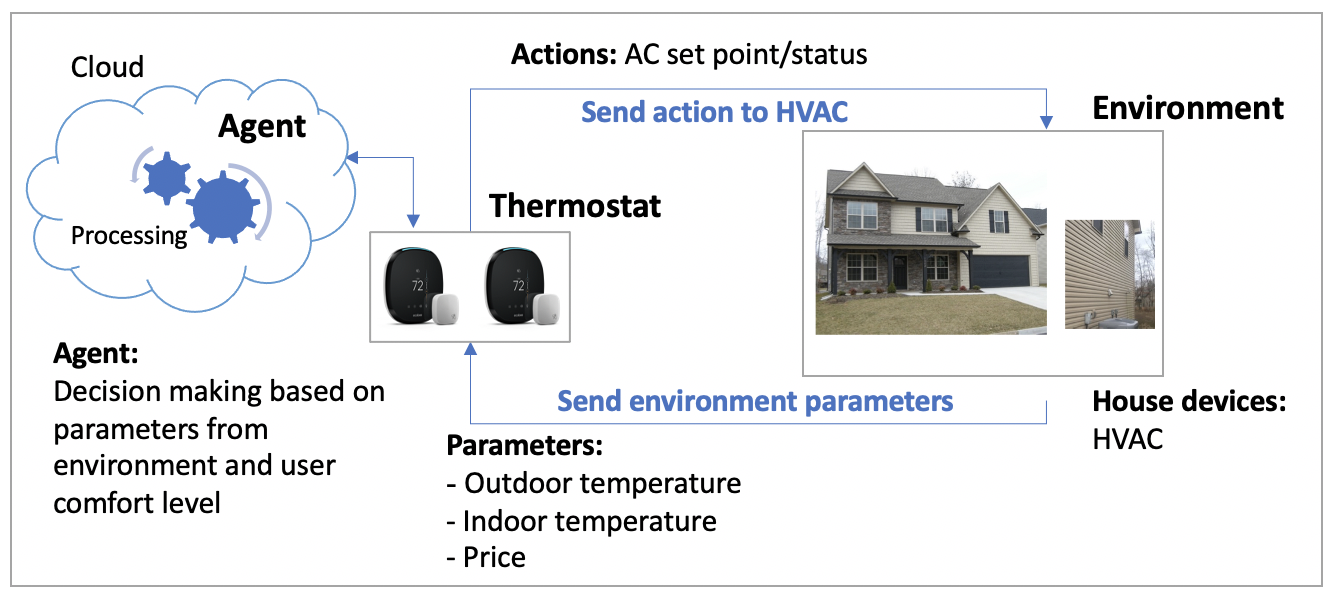
\includegraphics[width=1.0\columnwidth]{usecase/hvac_general.png}
\caption{General view of HVAC-to-Cloud system \cite{kotevska2020rl}}
\label{fig:hvac_general}
\end{figure}

\paragraph*{System model.}
User comfort level is defined as the allowed temperature range in the house, the range can remain constant during the entire 24 hour cycle, or it can vary based on the time of the day or the day of the week. Since the temperature in the house is affected by the outdoor temperature our goal is to keep the internal temperature within the desired user comfort level. 
Energy prices fluctuate through out the day, driven by market dynamics. We describe the pricing function as a sequence of values $Price = {P_1, P_2, . . . , P_m}$ where $P_i$ corresponds to the price at time slot $i$. At each time slot, the service provider determines the electricity price and charges the customer at the given rate. We determine the user cost based on the price and energy consumption during the time slot. At time $t_{k-1}$, we observe the set of all variables of the system which includes information about the outdoor temperature, the indoor temperature, and the pricing. Based on all this information, the  algorithm makes a dynamic decision to set the HVAC set point. This represents the HVAC state in the next time-interval $t_k$. After executing the HVAC setpoint action, we observe the system during time step $t_k$. These steps are executed in periodic intervals, as presented in Figure \ref{fig:hvac_general} and the setpoint recommendation process require advanced machine learning algorithm (e.g, reinforcement learning) \cite{kotevska2020rl}. Accurate recommendations can save energy and reduce cost. We organized this functionality in three parts Environmental Forecasting (EF), Learning from the past, (LP), and Set-Point Recommendation (SPR). EF calculates weather temperature and price predictions. LP learns from the behavior in the past. SPR model calculates next set-point based on past experience and EF predictions. Figure \ref{fig:hvac_flowchart} shows the general modeling system flow chat. Reward is a function of temperature violation and cost. This function is specific to the algorithm that was used in this case reinforcement learning (RL). If the temperature is above the desired setpoint and energy cost is high the reward is negative. While if the temperature is within the setpoint range and the energy price is low the reward is positive. This allows the RL-based method to learn the optimal behavior through continuous interaction with a building environment and without referring to any prior model knowledge.
The results are presented on the home device interface and historic results are presented on the dashboard using the cloud-as-a-service option.

\begin{figure}[htb]
\centering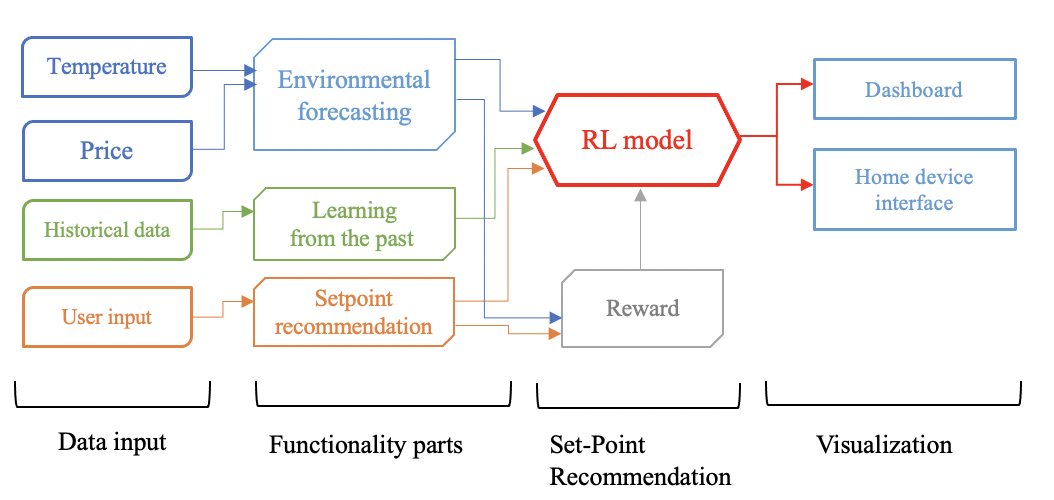
\includegraphics[width=1.0\columnwidth]{usecase/hvac_flowchart.png}
\caption{HVAC general modeling system flow chat.}
\label{fig:hvac_flowchart}
\end{figure}

\paragraph*{Functionalities and Activities} (based on Big Data Application Provider of NBDIF Ref. Architecture).

In this case study, we only focus on three main functionalities, namely EF, LP and SPR, and their activities. Figure \ref{fig:hvac_func_diagram} shows the cross-functional diagram for their actions.


\begin{figure}[htb]
\centering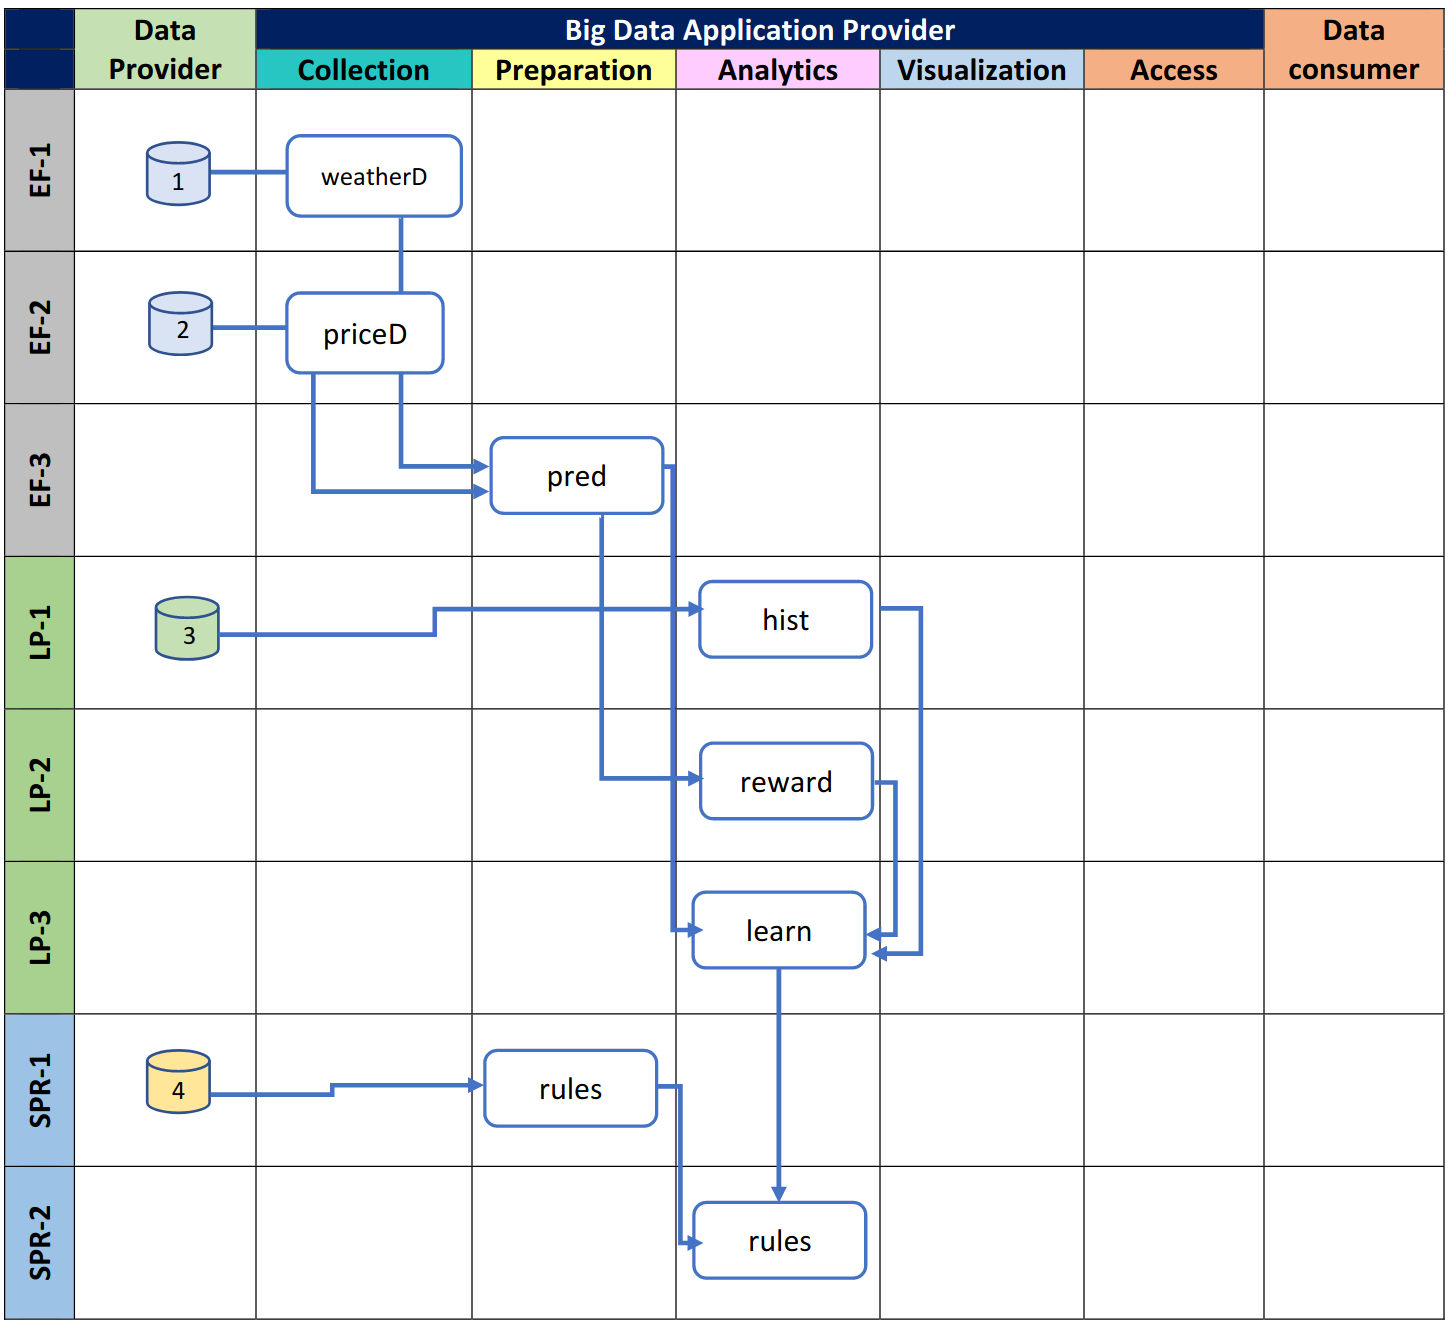
\includegraphics[width=1.0\columnwidth]{usecase/hvac_functional.png}
\caption{Cross-Functional Diagram HVAC Recommendation.}
\label{fig:hvac_func_diagram}
\end{figure}


EF Activities:

\begin{enumerate}
\item weatherD -- Collects current weather temperature and predicted temperature for timestamp X.
\item priceD -- Collects current electricity price and predicted price for timestamp X.
\item pred -- Extract needed data fields and packs it into an intermediate file format. Input data from the output of weatherD and priceD.
\end{enumerate}


LP Activities:

\begin{enumerate}
\item hist -- Prepares history data points and creates initial condition weights.
\item reward -- Generates reward based on the current weatherD and priceD.
\item learn -- Collects data from current weatherD, priced, reward.
\end{enumerate}

SPR Activities:

\begin{enumerate}
\item rules -- Creates rules based on user preferences and conversion preferences.
\item rlmodel --  Interpolates the output from learn, rules and generates set point recommendation.
\end{enumerate}

This setup is a general setup that is applicable to one-zone models. Results have shown that RL model has high generalization and adaptability to unseen environments, which indicates its practicability for real-world implementation \cite{du2021intelligent}.

The same functionality can be used with different building models and retail price models \cite{du2021intelligent}. 

%\paragraph*{Algorithm}

%\TODO{No datasets provided.}

This use case has the implicit requirements needing the following
aspects to be addressed by the framework we develop.

\begin{enumerate}

\item{\bf AS vendor neutral cloud and computer service integration.} ...

  \begin{enumerate}
    \item {\bf AS in cloud.} ...
    \item {\bf AS in LCCF.} ...
    \item {\bf AS in microservices.} ...
  \end{enumerate}

\item{\bf AS architecture.} ...

  \begin{enumerate}
    \item{\bf AS vendor neutral interfaces.} ...
    \item{\bf AS REST.} ...
    \item{\bf AS layers such as interface, service layer, and provider layer.} ...
  \end{enumerate}

\item{\bf AS workflow.} ...

  \begin{enumerate}
    \item{\bf AS catalog and registry.} ...
    \item{\bf AS cooperation.} ...
    \item{\bf competition.} ...
    \item{\bf AS orchestrator.} ...
  \end{enumerate}


\item{\bf AS calculation.}

  \begin{enumerate}
    \item{\bf AS with DL.} ...
    \item{\bf AS data analytics.} ...
  \end{enumerate}

\item{\bf AS security.} ...

\end{enumerate}


